\documentclass[a4paper,14pt]{extreport}
\usepackage[left=1.5cm,right=1.5cm,
    top=1.5cm,bottom=2cm,bindingoffset=0cm]{geometry}
\usepackage{scrextend}
\usepackage[T1,T2A]{fontenc}
\usepackage[utf8]{inputenc}
\linespread{1.5}
\usepackage[english,russian,ukrainian]{babel}
\usepackage{tabularx}
\usepackage{amssymb}
\usepackage{color}
\usepackage{amsmath}
\usepackage{mathrsfs}
\usepackage{listings}
\usepackage{graphicx}
\graphicspath{ {./images/} }
\usepackage{lipsum}
\usepackage{xcolor}
\usepackage{hyperref}
\usepackage{tcolorbox}
\usepackage{tikz}
\usepackage[framemethod=TikZ]{mdframed}
\usepackage{wrapfig,boxedminipage,lipsum}
\mdfdefinestyle{MyFrame}{%
linecolor=blue,outerlinewidth=2pt,roundcorner=20pt,innertopmargin=\baselineskip,innerbottommargin=\baselineskip,innerrightmargin=20pt,innerleftmargin=20pt,backgroundcolor=gray!50!white}
 \usepackage{csvsimple}
 \usepackage{supertabular}
\usepackage{pdflscape}
\usepackage{fancyvrb}
%\usepackage{comment}
\usepackage{array,tabularx}
\usepackage{colortbl}

\usepackage{varwidth}
\tcbuselibrary{skins}
\usepackage{fancybox}


\usepackage{tikz}
\usepackage[framemethod=TikZ]{mdframed}
\usepackage{xcolor}
\usetikzlibrary{calc}
\makeatletter
\newlength{\mylength}
\xdef\CircleFactor{1.1}
\setlength\mylength{\dimexpr\f@size pt}
\newsavebox{\mybox}
\newcommand*\circled[2][draw=blue]{\savebox\mybox{\vbox{\vphantom{WL1/}#1}}\setlength\mylength{\dimexpr\CircleFactor\dimexpr\ht\mybox+\dp\mybox\relax\relax}\tikzset{mystyle/.style={circle,#1,minimum height={\mylength}}}
\tikz[baseline=(char.base)]
\node[mystyle] (char) {#2};}
\makeatother

\definecolor{ggreen}{rgb}{0.4,1,0}
\definecolor{rred}{rgb}{1,0.1,0.1}
\definecolor{amber}{rgb}{1.0, 0.75, 0.0}
\definecolor{babyblue}{rgb}{0.54, 0.81, 0.94}
\definecolor{amethyst}{rgb}{0.6, 0.4, 0.8}
\usepackage{graphicx}
\usepackage{float}
\usepackage{wrapfig}
\usepackage{framed}
%for nice Code{
\lstdefinestyle{customc}{
  belowcaptionskip=1\baselineskip,
  breaklines=true,
  frame=L,
  xleftmargin=\parindent,
  language=C,
  showstringspaces=false,
  basicstyle=\small\ttfamily,
  keywordstyle=\bfseries\color{green!40!black},
  commentstyle=\itshape\color{purple!40!black},
  identifierstyle=\color{blue},
  stringstyle=\color{orange},
}
\lstset{escapechar=@,style=customc}
%}


\begin{document}
\pagecolor{white}

%----------------------------------------1
\newtcbox{\xmybox}[1][red]{on line, arc=7pt,colback=#1!10!white,colframe=#1!50!black, before upper={\rule[-3pt]{0pt}{10pt}},boxrule=1pt, boxsep=0pt,left=6pt,right=6pt,top=2pt,bottom=2pt}

\begin{titlepage}
  \begin{center}
    \large
    Національний технічний університет України \\ "Київський політехнічний інститут імені Ігоря Сікорського"


    Факультет Електроніки

    Кафедра мікроелектроніки
    \vfill

    \textsc{ЗВІТ}\\

    {\Large Про виконання курсової роботи \\
      з дисципліни: «Твердотільна електроніка-3»\\[1cm]

        Варіант №50


    }
  \bigskip
\end{center}
\vfill

\newlength{\ML}
\settowidth{\ML}{«\underline{\hspace{0.4cm}}» \underline{\hspace{2cm}}}
\hfill
\begin{minipage}{1\textwidth}
Виконавець:\\
Студент 3-го курсу \hspace{4cm} $\underset{\text{(підпис)}}{\underline{\hspace{0.2\textwidth}}}$  \hspace{1cm}А.\,С.~Мнацаканов\\
\vspace{1cm}

Перевірив: \hspace{6.1cm} $\underset{\text{(підпис)}}{\underline{\hspace{0.2\textwidth}}}$  \hspace{1cm}Л.\,М.~Королевич\\

\end{minipage}

\vfill

\begin{center}
2021
\end{center}
\end{titlepage}

\newpage
\setcounter{page}{2}


\begin{center}
    \textbf{Завдання}
\end{center}
Розрахувати геометричні розміри транзисторів


\begin{center}
  \textbf{Виконання завдання}
\end{center}

\begin{figure}[h!]
\center{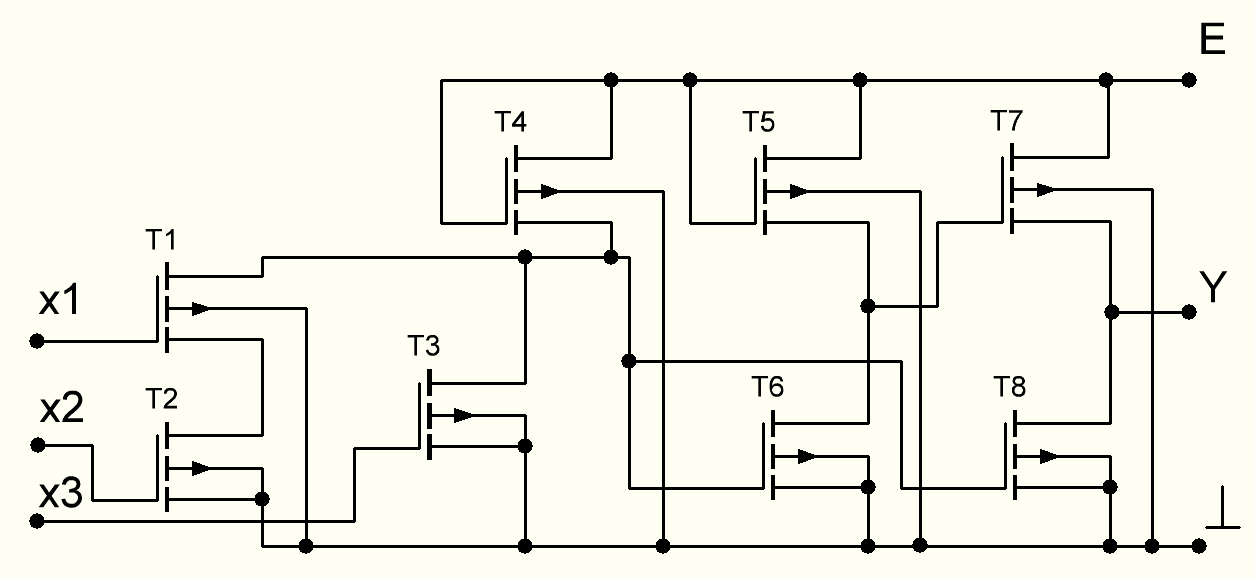
\includegraphics[width=1\linewidth]{1.png}}
\caption{Прототип схеми.}
\label{ris1}
\end{figure}

Перш за все запишу всі константи, які знадобляться:\\
\vspace{0.2cm}
\begin{minipage}{0.5\textwidth}
    \begin{flushleft}
  	\vspace{0.2cm}
  $\varepsilon_{0}=8,85 \cdot 10^{-14} \text{ }\dfrac{\text{Ф}}{\text{см}}$\\
  \vspace{0.2cm}
  $\varepsilon_{ox}=3,9$\\
  \vspace{0.2cm}
  $\varepsilon_{S}=11,8$\\
  \vspace{0.2cm}
  $ d_{o x}=100 \text{ } \text{нм}$\\
  \vspace{0.2cm}
  $ N_{B}=8,3 \cdot 10^{14}\text{ } \text{см}^{-3}$\\
  \vspace{0.2cm}
  $ U_{\text{nop.}}^{0}=-5,5 \text{ }\text{B}$\\
  \vspace{0.2cm}
  $ U_{n}=-12 \text{ }\text{B}$\\
  \vspace{0.2cm}
  $U^{0}=-1,1 \text{ }\text{B}$\\
  \vspace{0.2cm}
  $U^{1}=-10 \text{ }\text{~B}$\\
    \end{flushleft}
  \end{minipage}
  \begin{minipage}{0.3\textwidth}
    \begin{flushright}
    $\phi_{F}=0,283 B$\\
    \vspace{0.2cm}
    $C_{ox}=3,45 \cdot 10^{-8} \text{ }\dfrac{\text{Ф}}{\text{см}^{2}}$\\
    \vspace{0.2cm}
    $\mu_{p} = 225 \text{ }\dfrac{\text{см}^{2}}{\text{B}\cdot\text{c}}$\\
    \vspace{0.2cm}
    $t_{\text{викл}} = 760 \text{ }\text{нс}$\\
    \vspace{0.2cm}
    $ t_{\text{вкл}}= 100 \text{ }\text{нс}$\\
    \vspace{0.2cm} 
    $ I_{\text {load }}= 430\text{ } \text{мкА}$\\
    \vspace{0.2cm}
    $ C_{\text {H}}= 29\text{ } \text{пФ}$\\
    \vspace{0.2cm}
    \end{flushright}
\end{minipage}




Розгляд данної задачі починаю з першого каскаду, маю 4 транзистори, які можна поділити на дві підгрупки: верхній транзистор, який грає роль навантаження, та нижній, який керує транзистором. Оскільки маю  2 паралельно з'єднаних транзистора T1 і T2 об’єдную в один TE, вийде, що ширина кожного буде відноситися як $W_{T_E} =  \dfrac{W_{T_1}}{2} = \dfrac{W_{T_2}}{2}$ = $W_{T_3}$.
Тому, використовую відношення через струм колектора з методички і переписую для мєго випадку:\\

\resizebox{.9\textwidth}{!}{%
$
i_{C}=\dfrac{\mu \cdot \varepsilon_{0} \cdot \varepsilon_{o x}}{d_{\alpha x}} \cdot \dfrac{W}{L} \cdot\left[\left(U_{3}-U_{n o p}\right) \cdot U_{C}-\dfrac{U_{C}^{2}}{2}\right] \Rightarrow
\dfrac{W_{E}}{L_{E}}=\dfrac{i_{C} \cdot d_{o x}}{\mu \cdot \varepsilon_{0} \cdot \varepsilon_{o x}} \cdot \dfrac{1}{\left[\left(U_{3}-U_{n o p}\right) \cdot U_{C}-\dfrac{U_{C}^{2}}{2}\right]}
$}

\begin{align*}
U_{\text {nop }}=U_{\text {nop }}^{0}+K \cdot \sqrt{2 \cdot \phi_{F}+U_{n}}-K \cdot \sqrt{2 \cdot \phi_{F}}=5,76 \text{ } B
\end{align*}

\begin{align*}
\dfrac{W_{E}}{L_{E}}=\dfrac{i_{C} \cdot d_{o x}}{\mu \cdot \varepsilon_{0} \cdot \varepsilon_{o x}} \cdot \dfrac{1}{\left[\left(U_{\text{вх}}-U_{\text {nop}}^{0}\right) \cdot U_{\text {вих }} -
\dfrac{U_{\text {\text{вих} }}^{2}}{2}\right]}=10,17
\end{align*}

Замість виходу напруга логічного гуля, а замість входу напруга логічної одиниці. Так як зразок КЕФ, всі напруги від’ємні, але для спрощення обчислень \fcolorbox{black}{red!20}{беруться абсолютні значення}.
Далі, треба обрати довжину каналу. Я обираю 5 мкм, аби фінальні значення не перевищували 500 мкм.


Тоді, $L_{T_{E}} = 5 \text{ мкм}, W_{T_{1}}=W_{T_{2}}=2 \cdot W_{T_{E}}\text{ } \text{ a }  \text{ }   W_{T_{3}}=W_{T_{E}}$, де $W_{T_{E}} = L_{T_{E}} \cdot 10,17 \approx 55 \text{мкм}$. Тоді, маємо: $W_{T_{1}} = W_{T_{2}} = 110 \text{ мкм}, W_{T_{3}} = 55 \text{ мкм}$ \\
Тепер рахунки для навантажувального транзистора Т4. Для нього треба використовувати передавальну характеристику.

\resizebox{.9\textwidth}{!}{
$
\dfrac{\mu \cdot \varepsilon_{0} \cdot \varepsilon_{o x}}{2 \cdot d_{o x}} \cdot \dfrac{W_{T_{H}}}{L_{T_{H}}} \cdot\left(\left(U_{n}-U_{\text{вих}}\right)-U_{n o p}\right)^{2}=\dfrac{\mu \cdot \varepsilon_{0} \cdot \varepsilon_{ox}}{d_{ox}} \cdot \dfrac{W_{T_{E}}}{L_{T_{E}}} \cdot\left(\left(U_{\text{вх}}-U_{n o p .0}\right) \cdot U_{вих}-\dfrac{U_{\text{вих}}^{2}}{2}\right)$}

$$
\dfrac{W_{T_{H}}}{L_{T_{H}}}=
\dfrac{2 \dfrac{W_{T_{E}}}{L_{T_E}} \cdot\left(\left(U_{\text{вх}}-U_{\text {nop. 0}}\right) \cdot U_{\text {вих }}-
\dfrac{U_{\text {вих }}^{2}}{2}\right)}{\left(\left(U_{n}-U_{\text{вих}}\right)-U_{\text {nop }}\right)^{2}}=4,19
$$

$$  K = d_{ox}\cdot \dfrac{\sqrt{2\varepsilon_s \varepsilon_0 q N_B }}{\varepsilon_0 \varepsilon_{ox}} = 0,48 \sqrt{B}  $$

$$ U_{nop} =  U_{nop}^0+K\sqrt{2\phi_F+U_n}-K\sqrt{2\phi_F}  = 5,76 $$ B 

Довжина канада буде однією для всіх  транзисторів. \\
Тоді $W_{T_{4}} =  L_{T_{4}} \cdot 4,19 \approx 25 \text{ мкм}$.

Другий каскад такий ж, як і перший, тому можна перенести розміри з першого каскаду  \\
$W_{T_{5}}=W_{T_{4}}=25  \text{ мкм}$\\
$W_{T_{6}}=W_{T_{E}}=55  \text{ мкм}$

Третій каскад рахую по динамічним характеристикам. Верхній рахую по часу  вимикання, а нижній по часу вмикання.\\
$U_{m a x}=U_{\text{вих}}-U_{n o p}^{0}-K \cdot \sqrt{U_{\text{вх}}-U_{n o p}^{0}}=4,37 $ В\\
$\bar{U}_{n o p}=U_{n o p}^{0}+K \cdot \sqrt{2 \cdot \phi_{F}+\dfrac{1}{2} \cdot\left(U_{\max }-U_{u c x}\right)}-K \cdot \sqrt{\phi_{F}}=5,85$ В


$t_{\text{викл}} = \dfrac{2\cdot C_H \cdot d_{ox} \cdot L_{T_{7}}}{\mu \cdot \varepsilon_0 \cdot \varepsilon_{ox} \cdot W_{T_{7}}} \cdot
\dfrac{U_{\text{мах}} - U_{\text{исх}}}{(U_{\text{вх}} - \bar{U}_{\text{пор}} - U_{\text{мах}})\cdot(U_{\text{вх}} - \bar{U}_{\text{пор}} - U_{\text{исх}})} \Rightarrow$

$ \dfrac{W_{T_{7}}}{L_{T_{7}}} =
\dfrac{2\cdot C_H \cdot d_{ox} }{\mu \cdot \varepsilon_0 \cdot \varepsilon_{ox} \cdot\mu} \cdot
\dfrac{U_{\text{мах}} - U_{\text{исх}}}{(U_{\text{вх}} - \bar{U}_{\text{пор}} - U_{\text{мах}})\cdot(U_{\text{вх}} - \bar{U}_{\text{пор}} - U_{\text{исх}})} = 10,2$,  \\

де  $U_{\text{исх}} = U_{\text{вх}}$\\

Оскільки відношення у мене < 1,  то $W_{T_{6}} = L_{T_{6}} \cdot 10,2 =  55$ мкм.\\

Для нижнього транзистора, керуючого, шукаю по часу включення.\\

\resizebox{.9\textwidth}{!}{%
$
t_{\text {вкл }}=\frac{C_{H} \cdot d_{\text {ох }} \cdot L_{T_{s}}}{\mu \cdot \varepsilon_{0} \cdot \varepsilon_{o x} \cdot W_{T_{8}}} \cdot \frac{1}{\left(U_{\text {вx }}-U_{\text {nop }}^{0}\right)} \cdot\left\{\frac{U_{\text {max }}-\left(U_{\text {ex }}-U_{\text {nop }}^{0}\right)}{U_{\text {вx }}-U_{\text {nop }}^{0}}+\frac{1}{2} \ln \left[\frac{2\left(U_{\text {вx }}-U_{\text {nop }}^{0}\right)-U_{\text {ocm }}}{U_{\text {ocm }}}\right]\right\} \Rightarrow
$}

$ \dfrac{W_{T_{8}}}{L_{T_{8}}} =6,06 \Rightarrow {W_{T_{8}}} = 6,06 \cdot 5 = 35 $ мкм






\begin{table}[h!]
\begin{center}
\caption{Відношення W/L та розміри для кожного транзистора.}
\begin{tabular}{|c|c|c|c|}

\hline             & W/L         & W           & L \\
\hline   T1        & 22          & $1 1 0$     & $5$ \\
\hline   T2        & 22          & $1 1 0$     & $5$ \\
\hline   T3        & $10,17$     & $55$       & $5$ \\
\hline   $T4$      & $4,19$      & $25$       & $5$ \\
\hline   $T5$      & $4,19$      & $25$       & $5$ \\
\hline   $T6$      & $10,17$     & $55$       & $5$ \\
\hline   $T7$      & $10,2$      & $55$         & $5$ \\
\hline   $T8$      & $6,06$      & $3 5$       & $5$ \\
\hline
\end{tabular}
\end{center}
\end{table}












\end{document}
